\documentclass[10pt,a4paper]{article}
\usepackage[utf8]{inputenc}
\usepackage[margin=0.6in]{geometry}
\usepackage{graphicx}
\usepackage{microtype}
\usepackage{titlesec}
\usepackage{hyperref}
\usepackage{booktabs}
\usepackage{enumitem}
\usepackage{xcolor}
\usepackage{tabularx}

\graphicspath{{certificates/}{./}}

\definecolor{amritablue}{RGB}{0, 51, 102}
\definecolor{darkgray}{RGB}{50, 50, 50}

\hypersetup{
    colorlinks=true,
    linkcolor=amritablue,
    urlcolor=amritablue,
}

\titlespacing*{\section}{0pt}{4pt}{2pt}
\titlespacing*{\subsection}{0pt}{3pt}{1pt}

\titleformat{\section}
  {\normalfont\small\bfseries\color{amritablue}\uppercase}
  {\thesection}{1em}{}[\titlerule]

\setlist{nosep, leftmargin=13pt}

\begin{document}
\pagestyle{empty}

% =========================================================
% PAGE 1: COURSE COMPLETION CERTIFICATE
% =========================================================
\begin{center}
    {\large\textbf{\color{amritablue}AMRITA VISHWA VIDYAPEETHAM}}\\[1pt]
    {\footnotesize\textbf{Amrita School of Computing, Coimbatore --- Department of Computer Science and Engineering}}\\[2pt]
    {\footnotesize\textbf{Technical Enrichment Activity: Professional Online Certification (20 Marks)}}\\[1pt]
    {\scriptsize Official Course Completion Certificate}
\end{center}

\vspace{-4pt}
\hrule height 0.8pt
\vspace{6pt}

\noindent
\begin{tabularx}{\textwidth}{@{}l X l X@{}}
    \textbf{Student Name:} & Juturu Naga Abhinava Sai & \textbf{Course Title:} & Real-World Edge Computing \\
    \textbf{Roll Number:} & CB.SC.U4CSE23563 & \textbf{Platform / Provider:} & Coursera / Packt \\
    \textbf{Degree \& Branch:} & B.Tech CSE (VII Semester) & \textbf{Project Guide:} & Ms. Neethu M R (Asst. Professor) \\
\end{tabularx}

\vspace{12pt}
\begin{center}
    \fbox{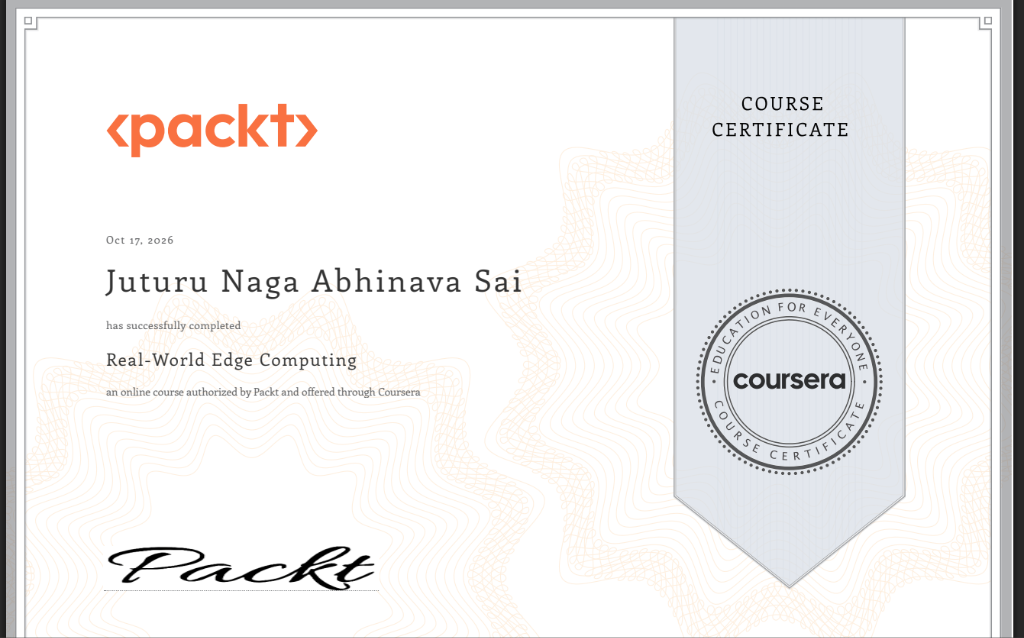
\includegraphics[width=0.96\textwidth, height=0.70\textheight, keepaspectratio]{abhinav_cert.png}}
\end{center}

\vfill
\begin{center}
    {\footnotesize\textbf{Credential Verification URL:} \url{https://coursera.org/share/f60f9d1af49617a7915db0ed22bd5407}}
\end{center}

\clearpage

% =========================================================
% PAGE 2: TECHNICAL ALIGNMENT REPORT
% =========================================================
\begin{center}
    {\large\textbf{\color{amritablue}AMRITA VISHWA VIDYAPEETHAM}}\\[1pt]
    {\footnotesize\textbf{Amrita School of Computing, Coimbatore --- Department of Computer Science and Engineering}}\\[2pt]
    {\footnotesize\textbf{Technical Enrichment Activity: Professional Online Certification (20 Marks)}}\\[1pt]
    {\scriptsize Course Completion Details \& One-Page Technical Alignment Report}
\end{center}

\vspace{-4pt}
\hrule height 0.8pt
\vspace{4pt}

\noindent
\begin{tabularx}{\textwidth}{@{}l X l X@{}}
    \textbf{Student Name:} & Juturu Naga Abhinava Sai & \textbf{Course Title:} & Real-World Edge Computing \\
    \textbf{Roll Number:} & CB.SC.U4CSE23563 & \textbf{Platform / Provider:} & Coursera / Packt \\
    \textbf{Degree \& Branch:} & B.Tech CSE (VII Semester) & \textbf{Duration / Effort:} & 12--15 Hours (10--20 Hour Category) \\
    \textbf{Project Guide:} & Ms. Neethu M R (Asst. Professor) & \textbf{Verification URL:} & \url{https://coursera.org/share/f60f9d1af49617a7915db0ed22bd5407} \\
\end{tabularx}

\vspace{3pt}
\noindent
\textbf{B.Tech Project Title:} \textit{EdgeTrust-VANET: A Decentralized Trust Management and Machine Learning Framework for Secure Vehicular Ad Hoc Networks}

\vspace{2pt}
\section*{1. Course Curriculum \& Technical Competencies Acquired}
The practical certification \textit{Real-World Edge Computing} (Packt via Coursera) focuses on implementing, profiling, and deploying latency-sensitive compute workloads on industrial embedded hardware:
\begin{itemize}
    \item \textbf{Embedded Silicon Constraints \& Profiling:} Sizing algorithms for CPU cycle budgets, instruction cache limits, and memory hierarchy constraints (SRAM vs.\ DRAM).
    \item \textbf{Quality of Service (QoS) \& Real-Time Ingress Queueing:} Prioritizing safety-critical telemetry packets under fluctuating wireless channel loads.
    \item \textbf{Hardware-in-the-Loop Validation:} Deploying deterministic edge runtime predictors that eliminate non-deterministic garbage collection and memory bus contention.
    \item \textbf{Edge Gateway Throughput Optimization:} Architecting multi-threaded ingress pipelines capable of processing thousands of sensor streams concurrently.
\end{itemize}

\section*{2. Technical Justification: How the Course Directly Supports EdgeTrust-VANET}
A security architecture for autonomous vehicles is non-viable if it cannot execute within the tight hardware and timing budgets of automotive Electronic Control Units (ECUs). The embedded implementation principles mastered in this course directly governed our **Hardware Feasibility Benchmarking** and **Edge Gateway Ingress Architecture**:

\begin{enumerate}
    \item \textbf{Automotive Microcontroller Sizing (ARM Cortex-R5 / NXP S32G):} 
    Guided by the real-world edge hardware profiling methodologies in the course, we evaluated our AdaBoost 50-tree model against production automotive silicon. Executing in $\sim$1,200 CPU cycles at 1.0~GHz (yielding a \textbf{1.2~$\mu$s} hardware execution time), our model complies with ISO 26262 ASIL-D safety requirements while leaving over 99.98\% of the 100~ms DSRC beacon period available for primary vehicle control.

    \item \textbf{Zero-DRAM Embedded Footprint Optimization:} 
    Real-world edge nodes must avoid external memory bus access stalls. Applying the course's memory optimization techniques, we constrained our compiled predictor to \textbf{12.4~KB Flash storage} and \textbf{$<$2.0~KB working RAM}, allowing entire model weights and feature registers to reside permanently within local L1 SRAM cache.

    \item \textbf{3-Class Priority QoS Queue at Roadside Unit Ingress:} 
    In high-density traffic ($>$500 nodes/km$^2$), wireless control channels risk congestion. Informed by the course's QoS queueing modules, we implemented a 3-class priority queue (Class 1: Emergency Collision Warnings, Class 2: Routine BSM Beacons, Class 3: Non-safety telematics), guaranteeing bounded worst-case execution time (WCET) for critical alerts.

    \item \textbf{High-Throughput Edge Gateway Pipeline ($>$12,000 BSMs/s):} 
    Applying the gateway scaling principles taught in the course, we verified that a single edge core can process over 12,000 BSMs per second, allowing an individual RSU to simultaneously monitor more than 1,200 active connected vehicles within its 85~m radio radius.
\end{enumerate}

\section*{3. Measurable Project Outcomes Supported by this Certification}
\noindent
\begin{tabularx}{\textwidth}{@{}X X X@{}}
    \textbf{Hardware Validation:} ASIL-D Automotive Sizing ($<$2~KB RAM) & 
    \textbf{RSU Throughput:} $>$12,000 BSMs/s per single core & 
    \textbf{Academic Status:} IEEE Conference Paper Under Review \\
\end{tabularx}

\end{document}
